\subsection{Estrutura do trabalho} \label{subsec:estrutura}
    Este trabalho está estruturado em~\ref{sec:conclusoes} capítulos, divididos da seguinte forma:
    
    \begin{figure}[H]
    	\centering
    	\caption{Estrutura da dissertação}
    	\label{fig:estrutura}
    	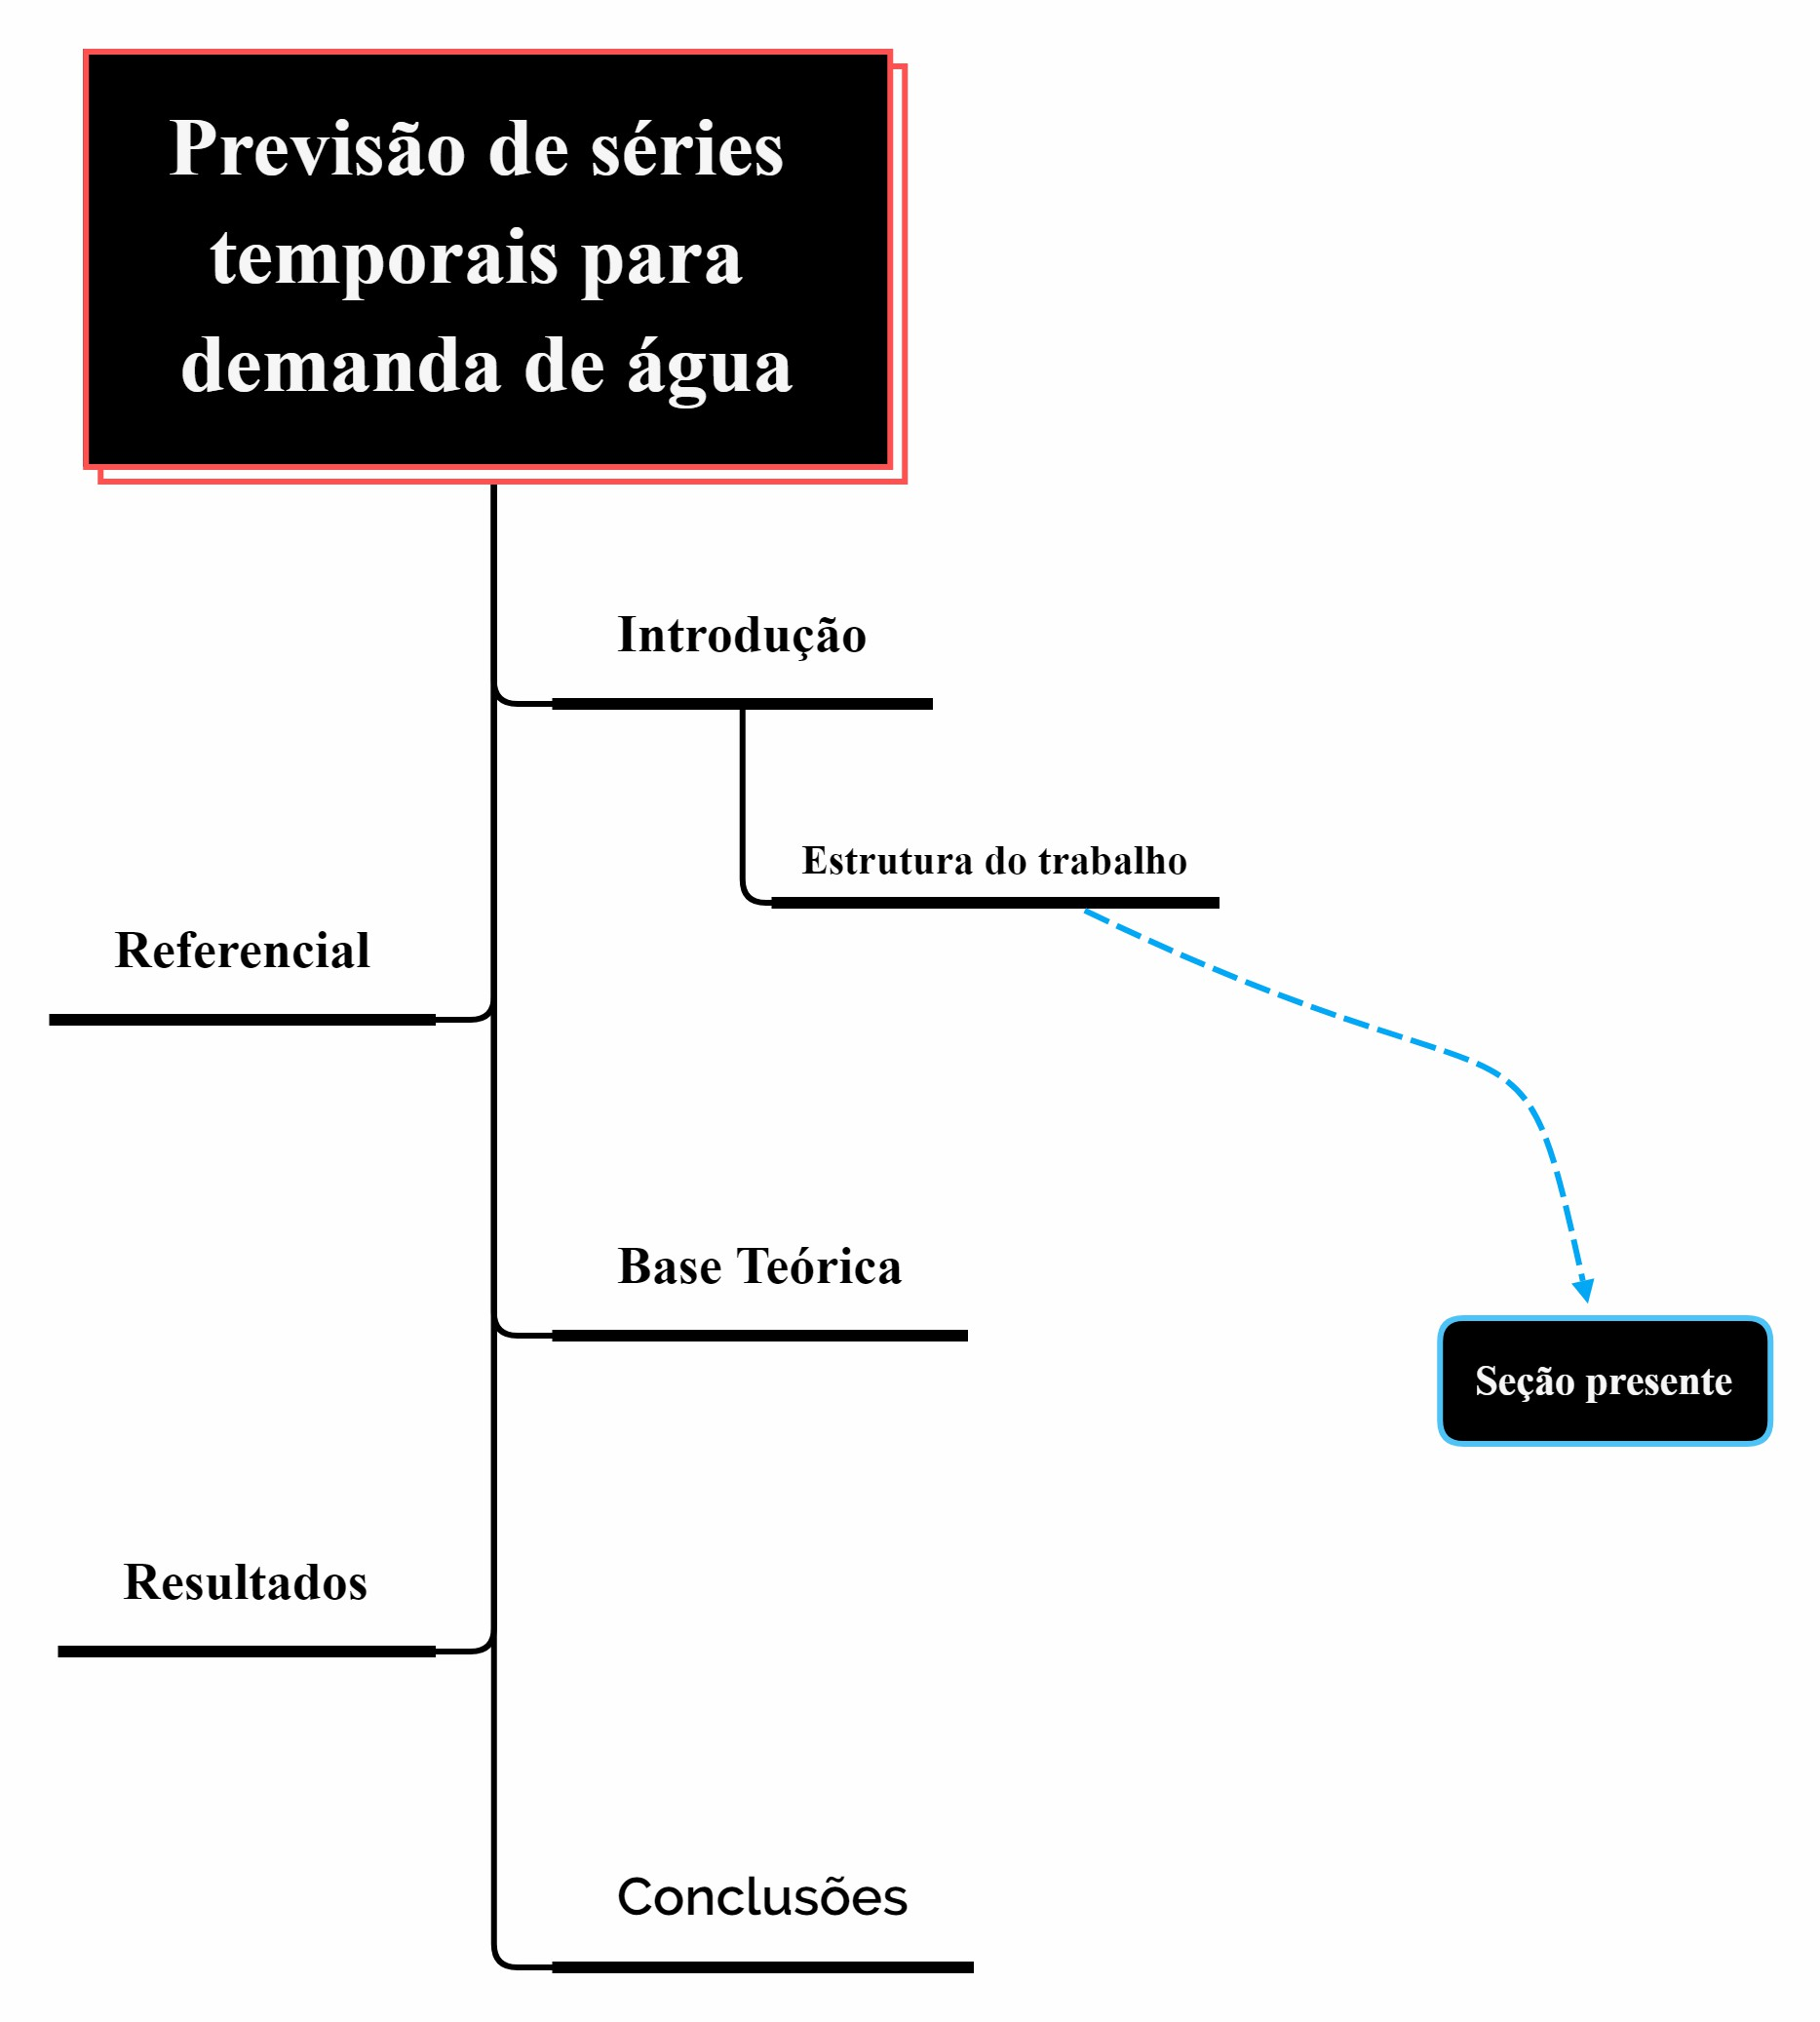
\includegraphics[width=0.7\linewidth]{Introducao/Figuras/Estrutura}
    	
    	Fonte: Elaboração própria 
    \end{figure}
        O capítulo~\ref{sec:int} apresenta a introdução do trabalho, contendo a contextualização, motivação, objetivo geral, os objetivos específicos, a metodologia utilizada, a justificativa da pesquisa, Contribuições, Publicações e a organização do trabalho.
        O capítulo~\ref{sec:refteo} apresenta a descrição do problema, revisão teórica do trabalho, fazendo um apanhado geral dos principais pesquisadores nos temas abordados na pesquisa.
        O capítulo~\ref{sec:base} apresenta os modelos que será trabalhado nos dados coletado.
        O capítulo~\ref{sec:result} apresenta os resultados da pesquisa, bem como uma análise dos resultados gerado.
        O capítulo~\ref{sec:conclusoes}, por fim, apresenta as considerações finais da pesquisa e algumas propostas de pesquisas futuras.